\section*{4/6/2562}

เนื่องจากเข้าทำงานเป็นวันแรก จึงต้องจัดสถานที่ทำงาน และทำงานต่อจากที่ได้รับมอบหมายก่อนการฝึกงาน

งานที่ได้รับมอบหมายโดยคร่าวคือการวิเคราะห์สภาวะความง่วงในคน โดยศึกษาจากกลุ่มเป้าหมายของพนักงานบริษัท
ซึ่งอาจารย์ที่ปรึกษาให้สิทธิ์ในการกำหนดแนวทางการวิเคราะห์ได้โดยอิสระ อย่างไรก็ตามงานของการวิเคราะห์ความง่วง
โดยตั้งต้นนั้นมักใช้การวิเคราะห์ภาพจากดวงตา (gaze monitoring) ซึ่งใช้วันนี้ในการหางานวิจัยตั้งต้น

นอกจากนี้ยังศึกษาแนวทาง ข้อกำหนด และมาตรฐานจริยธรรมในการทดลองภายในมนุษย์ (human subject research)

\section*{5/6/2562}

ศึกษาแนวทางในการทำ eye gazing ตามหนังสือที่ได้รับมอบหมาย และนำเสนองานวิจัยต่อจากที่เลือกจากเมื่อวาน

ปรับแก้แนวทางในการวิจัย และได้รับมอบหมายให้ออกแบบวิธีการทดลองโดยคร่าว
หารือกับทีมโปรแกรมเมอร์ว่าด้วยซอฟต์แวร์สำหรับการทดลอง

\section*{6/6/2562}

ศึกษาอุปกรณ์สำหรับติดตามดวงตา (Gazepoint) ก่อนจะพบว่าอุปกรณ์มีข้อจำกัดในการทำงานบางส่วน ทำให้ไม่สามารถดึง
ภาพดวงตาออกมาใช้ในโปรแกรมภายนอกได้ และติดต่อกับผู้ผลิตอุปกรณ์เพื่อหารือความเป็นไปได้ในการดึงภาพดวงตา

ศึกษาการใช้ Pytorch ในการทำการเรียนรู้เชิงลึก (deep learning) แทนที่ Keras

\section*{7/6/2562}

เปลี่ยนแนวทางการทำวิจัยด้วยข้อจำกัดของอุปกรณ์ มาเป็นการทำวิจัยบนกล้ามเนื้อตา (EOG) ค้นคว้าและทบทวนวรรรณกรรม
ที่เกี่ยวข้องกับงาน

ทำแบบทดสอบสำหรับบทเรียนจริยธรรมการวิจัยในมนุษย์จนอยู่ในเกณฑ์ได้รับประกาศนียบัตรผ่านการอบรม

\section*{10/6/2562}

นักเรียนจากโครงการพัฒนาอัจฉริยภาพทางวิทยาศาสตร์เข้ามาร่วมในทีม โดยการทดลองในส่วนของ Drowsiness research
ถูกแบ่งออกเป็นสองงานที่ต้องทดลองร่วมกัน จึงต้องตกลงแนวทางการทดลองให้ชัดเจน

ทดลองให้นักเรียนดังกล่าวศึกษาการวัดคลื่นสมองโดยอุปกรณ์ OpenBCI, ให้คำแนะนำถึงการเตรียมผิวหนัง (skin preparation)
ก่อนการติดอิเล็กโทรด, การเลือกใช้ชนิดอิเล็กโทรดและข้อดี-ข้อเสียของอิเล็กโทรดแต่ละชนิด

\section*{11/6/2562}

ทำงานที่ได้รับมอบหมายต่อจากเมื่อวาน

\section*{12/6/2562}

นัดประชุมงานกับอาจารย์ที่ปรึกษาโครงการ สรุปแนวทางการทดลอง และตัดสินใจเพิ่มการวัด PVT (Psychomotor vigilance task)
เพิ่มเติมในการทดลอง

เขียนโปรแกรมสำหรับทดสอบ PVT โดยใช้การสื่อสารบนอุปกรณ์หลายเครื่องเพื่อลดความจำเป็นในการซื้อปุ่ม (physical button)
ด้วยเหตุผลทางงบประมาณ

ช่วงเย็นรับประทานอาหารเย็นร่วมกับอาจารย์ธงชัย ชิวปรีชา

\section*{13/6/2562}

ได้รับมอบหมายให้ทดลองจับภาพตาเพื่อหา PERCLOS ด้วยกล้องเว็บแคมแบบที่มีหลอดอินฟราเรด ในเบื้องต้นสามารถครอปตัดเฉพาะส่วน
ที่เป็นลูกตาออกจากภาพใบหน้าแบบเต็มหน้าได้ อย่างไรก็ตาม ไม่ประสบความสำเร็จในการคำนวนร้อยละพื้นที่ของตาดำที่ไม่ถูกหนังตาบดบัง

\begin{figure}[H]
    \centering
    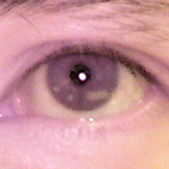
\includegraphics[width=0.4\textwidth]{images/268.png}
    \caption{ภาพถ่ายตาจากล้อง IR}
\end{figure}

\section*{14/6/2562}

ศึกษาและทบทวนวรรณกรรมว่าด้วยการประมวลผลภาพลูกตา และนำมาประยุกต์เขียนบนไลบรารี่ OpenCV จนสามารถสกัดตำแหน่งงของตาออกมา
จากภาพถ่ายของใบหน้าผู้ใช้ได้

ตัดสินใจเปลี่ยนจากเว็บแคมพร้อมหลอด IR เป็นกล้องธรรมดา

\begin{figure}[H]
    \centering
    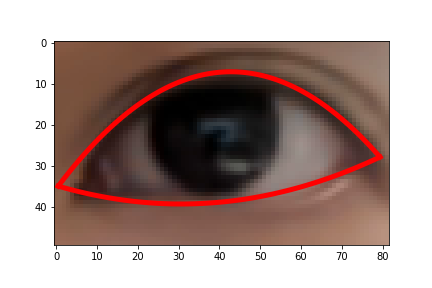
\includegraphics[width=0.4\textwidth]{images/111.png}
    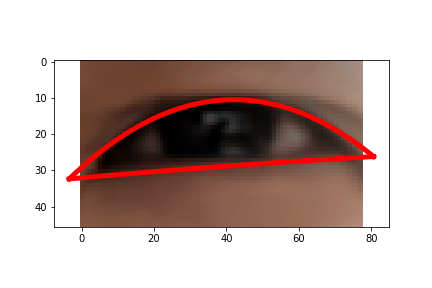
\includegraphics[width=0.4\textwidth]{images/171.png}
    \caption{ภาพถ่ายตาจากล้องที่ประมวลผลภาพเพื่อหาตำแหน่งของดวงตา ทั้งกรณีที่เปิดและปิดตา โดยประมวลผลภาพออกมาเป็นที่เรียบร้อย}
\end{figure}

\section*{17/6/2562}

ได้รับมอบหมายกระทันหันให้ร่วมเขียนเปเปอร์กับทีม SSVEP จีงเปลี่ยนสโคปงานเป็นการเขียนเปเปอร์ให้สามารถส่งตีพิมพ์ได้เร็วที่สุด

ศึกษาการใช้งานเครื่องมือทางสถิติ และทบทวนวรรณกรรมเท่าที่จำเป็น

\section*{18/6/2562}

เขียน ทบทวน และตรวจทานงานวิจัย

\section*{19/6/2562}

เขียน ทบทวน และตรวจทานงานวิจัยต่อ

\section*{20/6/2562}

เขียน ทบทวน และตรวจทานงานวิจัยต่อ

\section*{21/6/2562}

เขียน ทบทวน และตรวจทานงานวิจัยต่อ

\section*{24/6/2562}

เขียน ทบทวน และตรวจทานงานวิจัยต่อ

\section*{25/6/2562}

เขียน ทบทวน และตรวจทานงานวิจัยต่อ

\section*{26/6/2562}

เขียน ทบทวน และตรวจทานงานวิจัยต่อ

\section*{27/6/2562}

เขียน ทบทวน และตรวจทานงานวิจัยต่อ

\section*{28/6/2562}

เขียน ทบทวน และตรวจทานงานวิจัยต่อ

\section*{1/7/2562}

กลับมาทำงานในส่วนของการตรวจจับความง่วง ทดสอบเครื่องมือในการตรวจสอบความง่วงผ่านดวงตา

\section*{2/7/2562}

ประชุมรวมของห้องปฏิบัติการ และเขียนเอกสารการวิจัยในมนุษย์

\section*{3/7/2562}

ทบทวนวรรณกรรมสำหรับการตรวจจับความง่วง

\section*{4/7/2562}

ทบทวนวรรณกรรมสำหรับการตรวจจับความง่วง

\section*{5/7/2562}

ทบทวนวรรณกรรมสำหรับการตรวจจับความง่วง

\section*{8/7/2562}

ฟังบรรยายจาก Professor Guan Cuntai, NTU, SG

\section*{9/7/2562}

พัฒนาตัวตรวจจับดวงตาสำหรับพิจารณาความง่วงต่อ

\section*{10/7/2562}

พัฒนาตัวตรวจจับดวงตาสำหรับพิจารณาความง่วงต่อ

\section*{11/7/2562}

ประชุมกับนักประสาทวิทยาเพื่อปรับปรุงการทดลอง ปรับปรุงการทดลองต่อจากเมื่อวาน

\section*{12/7/2562}

ปรับปรุงการทดลองต่อจากเมื่อวาน

\section*{15/7/2562}

รันการทดลองครั้งแรกสำหรับการวิเคราะห์ความง่วง เพื่อทดลองหาข้อผิดพลาดจากการทำงาน

\section*{17/7/2562}

รันตัวประมวลผลวิดีโอสำหรับการทดลอง

งานวิจัยที่ส่งตีพิมพ์ได้รับการตีกลับ จึงได้รับมอบหมายให้นำมาปรับทวนงานวิจัย และตรวจสอบงานใหม่

\section*{18/7/2562}

ทดลองหาความสัมพันธ์บนชุดข้อมูลที่ได้จากการทดลอง

\section*{19/7/2562}

ทดลองหาความสัมพันธ์บนชุดข้อมูลที่ได้จากการทดลอง

\section*{22/7/2562}

ทดลองหาความสัมพันธ์บนชุดข้อมูลที่ได้จากการทดลอง

\section*{23/7/2562}

เขียน ทบทวน และตรวจทานงานวิจัยต่อ

\section*{24/7/2562}

เขียน ทบทวน และตรวจทานงานวิจัยต่อ

\section*{30/7/2562}

ทดลองหาความสัมพันธ์บนชุดข้อมูลที่ได้จากการทดลอง ประชุมโดยกระชับเพื่อสรุปแนวทางการออกแบบการทดลอง

\section*{30/7/2562}

ปรับแก้การทดลองตามที่ประชุม สรุปแนวทางการทดลองใหม่เป็นฉบับสมบูรณ์